% !TeX spellcheck = sk_SK-Slovak
\documentclass[a4paper]{article}
\usepackage[slovak]{babel}
\usepackage[utf8]{inputenc}
\usepackage[T1]{fontenc}
\usepackage{a4wide}
\usepackage{amsmath}
\usepackage{amsfonts}
\usepackage{amssymb}
\usepackage{mathrsfs}
\usepackage[small,bf]{caption}
\usepackage{subcaption}
\usepackage{xcolor}
\usepackage{graphicx}
\usepackage{enumerate}
\usepackage{hyperref}
\usepackage{fancyvrb}
\usepackage{listings}
%\usepackage{lstautogobble}
\usepackage{stmaryrd}

\lstset{basicstyle=\ttfamily,
	mathescape=true,
	escapeinside=||%,
	%autogobble
}


\fvset{tabsize=4}


\pagestyle{empty}
\setlength{\parindent}{0pt}

\newenvironment{modenumerate}
{\enumerate\setupmodenumerate}
{\endenumerate}

\newif\ifmoditem
\newcommand{\setupmodenumerate}{%
	\global\moditemfalse
	\let\origmakelabel\makelabel
	\def\moditem##1{\global\moditemtrue\def\mesymbol{##1}\item}%
	\def\makelabel##1{%
		\origmakelabel{##1\ifmoditem\rlap{\mesymbol}\fi\enspace}%
		\global\moditemfalse}%
}

\makeatletter
\def\@seccntformat#1{%
	\expandafter\ifx\csname c@#1\endcsname\c@section\else
	\csname the#1\endcsname\quad
	\fi}
\makeatother

\begin{document} 
	
\pagenumbering{arabic}
\pagestyle{plain}

\begin{center}
	\sc\large
	Formálne metódy tvorby softvéru\\
	Domáca úloha 4 
\end{center}

Autor: Marián Kravec

\section{1.)}

\begin{figure}[!h]
	\centering
	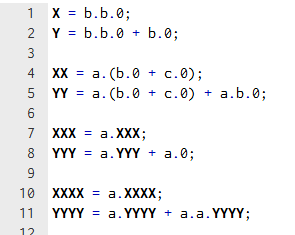
\includegraphics[width=0.55\textwidth]{proc_1.png}
	\caption{Zadané procesy}
\end{figure}

d. spĺňa silnú bisimuláciu takže ak tomu správne rozumiem nemala by existovať formula ktorá ich rozlišuje, čiže buď som niečo zle napísal, niečomu zle porozumel alebo je to chyták...

\begin{figure}[!h]
	\centering
	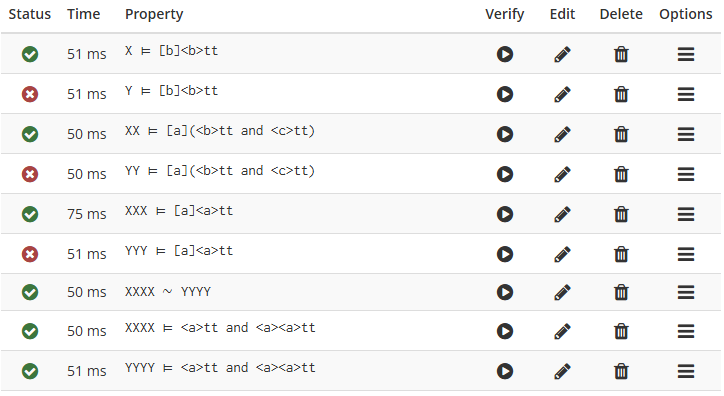
\includegraphics[width=1\textwidth]{form_1.png}
	\caption{Vymyslené formuly}
\end{figure}


\section{2.)}

Zväčša pomerne primitívne len aby formulu splnili, občas niečo pridané len tak.

\begin{figure}[!h]
	\centering
	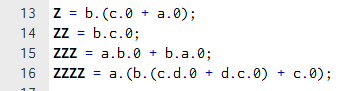
\includegraphics[width=0.6\textwidth]{proc_2.png}
	\caption{Vymyslené procesy}
\end{figure}


\begin{figure}[!h]
	\centering
	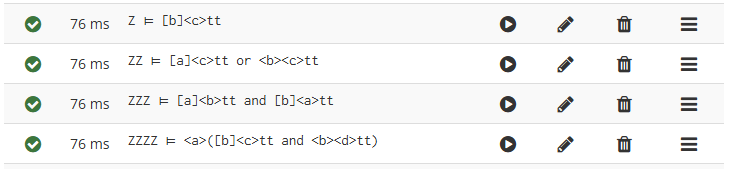
\includegraphics[width=1\textwidth]{form_2.png}
	\caption{Kontrola splnenia formúl}
\end{figure}

\end{document}